% Created by tikzDevice version 0.10.1 on 2017-11-26 21:02:42
% !TEX encoding = UTF-8 Unicode
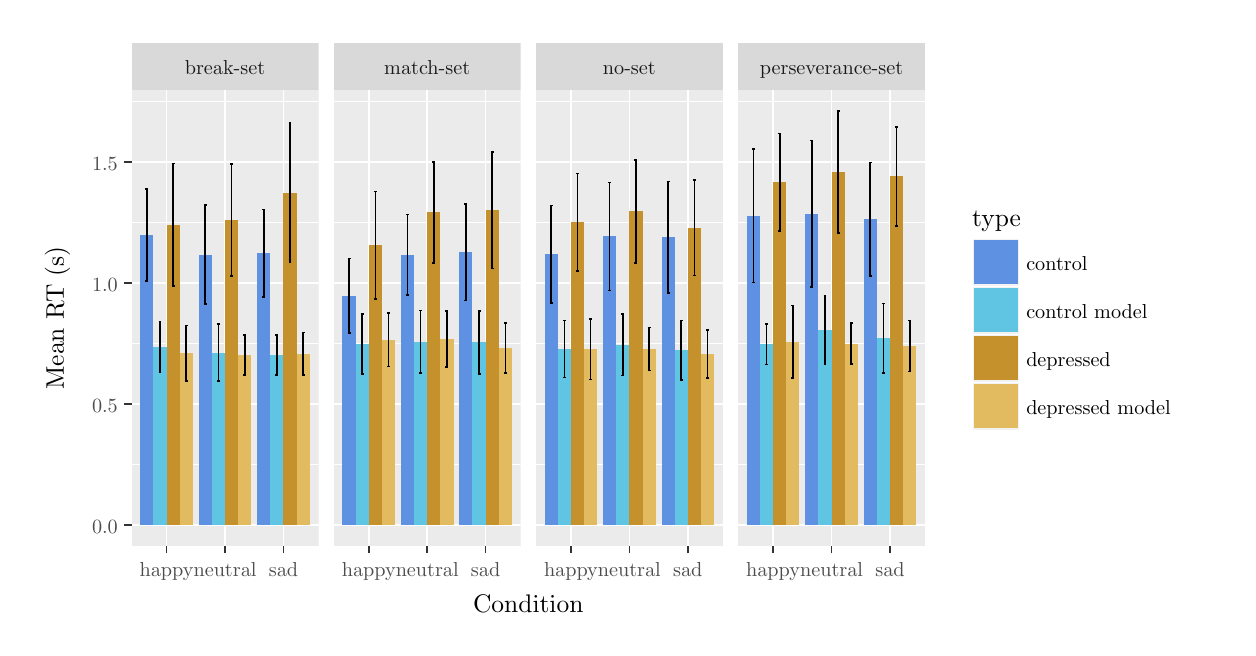
\begin{tikzpicture}[x=1pt,y=1pt]
\definecolor{fillColor}{RGB}{255,255,255}
\path[use as bounding box,fill=fillColor,fill opacity=0.00] (0,0) rectangle (433.62,216.81);
\begin{scope}
\path[clip] (  0.00,  0.00) rectangle (433.62,216.81);
\definecolor{drawColor}{RGB}{255,255,255}
\definecolor{fillColor}{RGB}{255,255,255}

\path[draw=drawColor,line width= 0.6pt,line join=round,line cap=round,fill=fillColor] (  0.00,  0.00) rectangle (433.62,216.81);
\end{scope}
\begin{scope}
\path[clip] ( 37.53, 29.59) rectangle (105.09,194.25);
\definecolor{fillColor}{gray}{0.92}

\path[fill=fillColor] ( 37.53, 29.59) rectangle (105.09,194.25);
\definecolor{drawColor}{RGB}{255,255,255}

\path[draw=drawColor,line width= 0.3pt,line join=round] ( 37.53, 58.93) --
	(105.09, 58.93);

\path[draw=drawColor,line width= 0.3pt,line join=round] ( 37.53,102.65) --
	(105.09,102.65);

\path[draw=drawColor,line width= 0.3pt,line join=round] ( 37.53,146.37) --
	(105.09,146.37);

\path[draw=drawColor,line width= 0.3pt,line join=round] ( 37.53,190.09) --
	(105.09,190.09);

\path[draw=drawColor,line width= 0.6pt,line join=round] ( 37.53, 37.07) --
	(105.09, 37.07);

\path[draw=drawColor,line width= 0.6pt,line join=round] ( 37.53, 80.79) --
	(105.09, 80.79);

\path[draw=drawColor,line width= 0.6pt,line join=round] ( 37.53,124.51) --
	(105.09,124.51);

\path[draw=drawColor,line width= 0.6pt,line join=round] ( 37.53,168.23) --
	(105.09,168.23);

\path[draw=drawColor,line width= 0.6pt,line join=round] ( 50.20, 29.59) --
	( 50.20,194.25);

\path[draw=drawColor,line width= 0.6pt,line join=round] ( 71.31, 29.59) --
	( 71.31,194.25);

\path[draw=drawColor,line width= 0.6pt,line join=round] ( 92.42, 29.59) --
	( 92.42,194.25);
\definecolor{fillColor}{RGB}{226,186,95}

\path[fill=fillColor] ( 54.95, 37.07) rectangle ( 59.70, 99.13);
\definecolor{fillColor}{RGB}{196,145,45}

\path[fill=fillColor] ( 50.20, 37.07) rectangle ( 54.95,145.58);
\definecolor{fillColor}{RGB}{95,197,226}

\path[fill=fillColor] ( 45.45, 37.07) rectangle ( 50.20,101.35);
\definecolor{fillColor}{RGB}{95,145,226}

\path[fill=fillColor] ( 40.70, 37.07) rectangle ( 45.45,141.91);
\definecolor{fillColor}{RGB}{226,186,95}

\path[fill=fillColor] ( 76.06, 37.07) rectangle ( 80.81, 98.49);
\definecolor{fillColor}{RGB}{196,145,45}

\path[fill=fillColor] ( 71.31, 37.07) rectangle ( 76.06,147.33);
\definecolor{fillColor}{RGB}{95,197,226}

\path[fill=fillColor] ( 66.56, 37.07) rectangle ( 71.31, 99.42);
\definecolor{fillColor}{RGB}{95,145,226}

\path[fill=fillColor] ( 61.81, 37.07) rectangle ( 66.56,134.83);
\definecolor{fillColor}{RGB}{226,186,95}

\path[fill=fillColor] ( 97.17, 37.07) rectangle (101.92, 99.05);
\definecolor{fillColor}{RGB}{196,145,45}

\path[fill=fillColor] ( 92.42, 37.07) rectangle ( 97.17,157.21);
\definecolor{fillColor}{RGB}{95,197,226}

\path[fill=fillColor] ( 87.67, 37.07) rectangle ( 92.42, 98.53);
\definecolor{fillColor}{RGB}{95,145,226}

\path[fill=fillColor] ( 82.92, 37.07) rectangle ( 87.67,135.26);
\definecolor{drawColor}{RGB}{0,0,0}

\path[draw=drawColor,line width= 0.6pt,line join=round] ( 56.80,109.20) --
	( 57.85,109.20);

\path[draw=drawColor,line width= 0.6pt,line join=round] ( 57.32,109.20) --
	( 57.32, 89.07);

\path[draw=drawColor,line width= 0.6pt,line join=round] ( 56.80, 89.07) --
	( 57.85, 89.07);

\path[draw=drawColor,line width= 0.6pt,line join=round] ( 52.05,167.70) --
	( 53.10,167.70);

\path[draw=drawColor,line width= 0.6pt,line join=round] ( 52.57,167.70) --
	( 52.57,123.46);

\path[draw=drawColor,line width= 0.6pt,line join=round] ( 52.05,123.46) --
	( 53.10,123.46);

\path[draw=drawColor,line width= 0.6pt,line join=round] ( 47.30,110.47) --
	( 48.35,110.47);

\path[draw=drawColor,line width= 0.6pt,line join=round] ( 47.82,110.47) --
	( 47.82, 92.22);

\path[draw=drawColor,line width= 0.6pt,line join=round] ( 47.30, 92.22) --
	( 48.35, 92.22);

\path[draw=drawColor,line width= 0.6pt,line join=round] ( 42.55,158.43) --
	( 43.60,158.43);

\path[draw=drawColor,line width= 0.6pt,line join=round] ( 43.07,158.43) --
	( 43.07,125.38);

\path[draw=drawColor,line width= 0.6pt,line join=round] ( 42.55,125.38) --
	( 43.60,125.38);

\path[draw=drawColor,line width= 0.6pt,line join=round] ( 77.91,105.64) --
	( 78.96,105.64);

\path[draw=drawColor,line width= 0.6pt,line join=round] ( 78.44,105.64) --
	( 78.44, 91.35);

\path[draw=drawColor,line width= 0.6pt,line join=round] ( 77.91, 91.35) --
	( 78.96, 91.35);

\path[draw=drawColor,line width= 0.6pt,line join=round] ( 73.16,167.62) --
	( 74.21,167.62);

\path[draw=drawColor,line width= 0.6pt,line join=round] ( 73.69,167.62) --
	( 73.69,127.04);

\path[draw=drawColor,line width= 0.6pt,line join=round] ( 73.16,127.04) --
	( 74.21,127.04);

\path[draw=drawColor,line width= 0.6pt,line join=round] ( 68.41,109.66) --
	( 69.46,109.66);

\path[draw=drawColor,line width= 0.6pt,line join=round] ( 68.94,109.66) --
	( 68.94, 89.17);

\path[draw=drawColor,line width= 0.6pt,line join=round] ( 68.41, 89.17) --
	( 69.46, 89.17);

\path[draw=drawColor,line width= 0.6pt,line join=round] ( 63.66,152.75) --
	( 64.71,152.75);

\path[draw=drawColor,line width= 0.6pt,line join=round] ( 64.19,152.75) --
	( 64.19,116.90);

\path[draw=drawColor,line width= 0.6pt,line join=round] ( 63.66,116.90) --
	( 64.71,116.90);

\path[draw=drawColor,line width= 0.6pt,line join=round] ( 99.02,106.72) --
	(100.07,106.72);

\path[draw=drawColor,line width= 0.6pt,line join=round] ( 99.55,106.72) --
	( 99.55, 91.38);

\path[draw=drawColor,line width= 0.6pt,line join=round] ( 99.02, 91.38) --
	(100.07, 91.38);

\path[draw=drawColor,line width= 0.6pt,line join=round] ( 94.27,182.39) --
	( 95.32,182.39);

\path[draw=drawColor,line width= 0.6pt,line join=round] ( 94.80,182.39) --
	( 94.80,132.03);

\path[draw=drawColor,line width= 0.6pt,line join=round] ( 94.27,132.03) --
	( 95.32,132.03);

\path[draw=drawColor,line width= 0.6pt,line join=round] ( 89.52,105.87) --
	( 90.57,105.87);

\path[draw=drawColor,line width= 0.6pt,line join=round] ( 90.05,105.87) --
	( 90.05, 91.19);

\path[draw=drawColor,line width= 0.6pt,line join=round] ( 89.52, 91.19) --
	( 90.57, 91.19);

\path[draw=drawColor,line width= 0.6pt,line join=round] ( 84.77,151.09) --
	( 85.82,151.09);

\path[draw=drawColor,line width= 0.6pt,line join=round] ( 85.30,151.09) --
	( 85.30,119.44);

\path[draw=drawColor,line width= 0.6pt,line join=round] ( 84.77,119.44) --
	( 85.82,119.44);
\end{scope}
\begin{scope}
\path[clip] (110.59, 29.59) rectangle (178.14,194.25);
\definecolor{fillColor}{gray}{0.92}

\path[fill=fillColor] (110.59, 29.59) rectangle (178.14,194.25);
\definecolor{drawColor}{RGB}{255,255,255}

\path[draw=drawColor,line width= 0.3pt,line join=round] (110.59, 58.93) --
	(178.14, 58.93);

\path[draw=drawColor,line width= 0.3pt,line join=round] (110.59,102.65) --
	(178.14,102.65);

\path[draw=drawColor,line width= 0.3pt,line join=round] (110.59,146.37) --
	(178.14,146.37);

\path[draw=drawColor,line width= 0.3pt,line join=round] (110.59,190.09) --
	(178.14,190.09);

\path[draw=drawColor,line width= 0.6pt,line join=round] (110.59, 37.07) --
	(178.14, 37.07);

\path[draw=drawColor,line width= 0.6pt,line join=round] (110.59, 80.79) --
	(178.14, 80.79);

\path[draw=drawColor,line width= 0.6pt,line join=round] (110.59,124.51) --
	(178.14,124.51);

\path[draw=drawColor,line width= 0.6pt,line join=round] (110.59,168.23) --
	(178.14,168.23);

\path[draw=drawColor,line width= 0.6pt,line join=round] (123.25, 29.59) --
	(123.25,194.25);

\path[draw=drawColor,line width= 0.6pt,line join=round] (144.37, 29.59) --
	(144.37,194.25);

\path[draw=drawColor,line width= 0.6pt,line join=round] (165.48, 29.59) --
	(165.48,194.25);
\definecolor{fillColor}{RGB}{226,186,95}

\path[fill=fillColor] (128.00, 37.07) rectangle (132.75,103.99);
\definecolor{fillColor}{RGB}{196,145,45}

\path[fill=fillColor] (123.25, 37.07) rectangle (128.00,138.15);
\definecolor{fillColor}{RGB}{95,197,226}

\path[fill=fillColor] (118.50, 37.07) rectangle (123.25,102.57);
\definecolor{fillColor}{RGB}{95,145,226}

\path[fill=fillColor] (113.75, 37.07) rectangle (118.50,119.96);
\definecolor{fillColor}{RGB}{226,186,95}

\path[fill=fillColor] (149.12, 37.07) rectangle (153.87,104.34);
\definecolor{fillColor}{RGB}{196,145,45}

\path[fill=fillColor] (144.37, 37.07) rectangle (149.12,150.04);
\definecolor{fillColor}{RGB}{95,197,226}

\path[fill=fillColor] (139.62, 37.07) rectangle (144.37,103.37);
\definecolor{fillColor}{RGB}{95,145,226}

\path[fill=fillColor] (134.87, 37.07) rectangle (139.62,134.74);
\definecolor{fillColor}{RGB}{226,186,95}

\path[fill=fillColor] (170.23, 37.07) rectangle (174.98,101.13);
\definecolor{fillColor}{RGB}{196,145,45}

\path[fill=fillColor] (165.48, 37.07) rectangle (170.23,150.92);
\definecolor{fillColor}{RGB}{95,197,226}

\path[fill=fillColor] (160.73, 37.07) rectangle (165.48,103.09);
\definecolor{fillColor}{RGB}{95,145,226}

\path[fill=fillColor] (155.98, 37.07) rectangle (160.73,135.61);
\definecolor{drawColor}{RGB}{0,0,0}

\path[draw=drawColor,line width= 0.6pt,line join=round] (129.85,113.64) --
	(130.91,113.64);

\path[draw=drawColor,line width= 0.6pt,line join=round] (130.38,113.64) --
	(130.38, 94.33);

\path[draw=drawColor,line width= 0.6pt,line join=round] (129.85, 94.33) --
	(130.91, 94.33);

\path[draw=drawColor,line width= 0.6pt,line join=round] (125.10,157.56) --
	(126.16,157.56);

\path[draw=drawColor,line width= 0.6pt,line join=round] (125.63,157.56) --
	(125.63,118.74);

\path[draw=drawColor,line width= 0.6pt,line join=round] (125.10,118.74) --
	(126.16,118.74);

\path[draw=drawColor,line width= 0.6pt,line join=round] (120.35,113.46) --
	(121.41,113.46);

\path[draw=drawColor,line width= 0.6pt,line join=round] (120.88,113.46) --
	(120.88, 91.67);

\path[draw=drawColor,line width= 0.6pt,line join=round] (120.35, 91.67) --
	(121.41, 91.67);

\path[draw=drawColor,line width= 0.6pt,line join=round] (115.60,133.43) --
	(116.66,133.43);

\path[draw=drawColor,line width= 0.6pt,line join=round] (116.13,133.43) --
	(116.13,106.50);

\path[draw=drawColor,line width= 0.6pt,line join=round] (115.60,106.50) --
	(116.66,106.50);

\path[draw=drawColor,line width= 0.6pt,line join=round] (150.96,114.45) --
	(152.02,114.45);

\path[draw=drawColor,line width= 0.6pt,line join=round] (151.49,114.45) --
	(151.49, 94.23);

\path[draw=drawColor,line width= 0.6pt,line join=round] (150.96, 94.23) --
	(152.02, 94.23);

\path[draw=drawColor,line width= 0.6pt,line join=round] (146.21,168.32) --
	(147.27,168.32);

\path[draw=drawColor,line width= 0.6pt,line join=round] (146.74,168.32) --
	(146.74,131.77);

\path[draw=drawColor,line width= 0.6pt,line join=round] (146.21,131.77) --
	(147.27,131.77);

\path[draw=drawColor,line width= 0.6pt,line join=round] (141.46,114.64) --
	(142.52,114.64);

\path[draw=drawColor,line width= 0.6pt,line join=round] (141.99,114.64) --
	(141.99, 92.09);

\path[draw=drawColor,line width= 0.6pt,line join=round] (141.46, 92.09) --
	(142.52, 92.09);

\path[draw=drawColor,line width= 0.6pt,line join=round] (136.71,149.34) --
	(137.77,149.34);

\path[draw=drawColor,line width= 0.6pt,line join=round] (137.24,149.34) --
	(137.24,120.14);

\path[draw=drawColor,line width= 0.6pt,line join=round] (136.71,120.14) --
	(137.77,120.14);

\path[draw=drawColor,line width= 0.6pt,line join=round] (172.07,110.19) --
	(173.13,110.19);

\path[draw=drawColor,line width= 0.6pt,line join=round] (172.60,110.19) --
	(172.60, 92.08);

\path[draw=drawColor,line width= 0.6pt,line join=round] (172.07, 92.08) --
	(173.13, 92.08);

\path[draw=drawColor,line width= 0.6pt,line join=round] (167.32,171.99) --
	(168.38,171.99);

\path[draw=drawColor,line width= 0.6pt,line join=round] (167.85,171.99) --
	(167.85,129.84);

\path[draw=drawColor,line width= 0.6pt,line join=round] (167.32,129.84) --
	(168.38,129.84);

\path[draw=drawColor,line width= 0.6pt,line join=round] (162.57,114.47) --
	(163.63,114.47);

\path[draw=drawColor,line width= 0.6pt,line join=round] (163.10,114.47) --
	(163.10, 91.71);

\path[draw=drawColor,line width= 0.6pt,line join=round] (162.57, 91.71) --
	(163.63, 91.71);

\path[draw=drawColor,line width= 0.6pt,line join=round] (157.82,153.01) --
	(158.88,153.01);

\path[draw=drawColor,line width= 0.6pt,line join=round] (158.35,153.01) --
	(158.35,118.21);

\path[draw=drawColor,line width= 0.6pt,line join=round] (157.82,118.21) --
	(158.88,118.21);
\end{scope}
\begin{scope}
\path[clip] (183.64, 29.59) rectangle (251.20,194.25);
\definecolor{fillColor}{gray}{0.92}

\path[fill=fillColor] (183.64, 29.59) rectangle (251.20,194.25);
\definecolor{drawColor}{RGB}{255,255,255}

\path[draw=drawColor,line width= 0.3pt,line join=round] (183.64, 58.93) --
	(251.20, 58.93);

\path[draw=drawColor,line width= 0.3pt,line join=round] (183.64,102.65) --
	(251.20,102.65);

\path[draw=drawColor,line width= 0.3pt,line join=round] (183.64,146.37) --
	(251.20,146.37);

\path[draw=drawColor,line width= 0.3pt,line join=round] (183.64,190.09) --
	(251.20,190.09);

\path[draw=drawColor,line width= 0.6pt,line join=round] (183.64, 37.07) --
	(251.20, 37.07);

\path[draw=drawColor,line width= 0.6pt,line join=round] (183.64, 80.79) --
	(251.20, 80.79);

\path[draw=drawColor,line width= 0.6pt,line join=round] (183.64,124.51) --
	(251.20,124.51);

\path[draw=drawColor,line width= 0.6pt,line join=round] (183.64,168.23) --
	(251.20,168.23);

\path[draw=drawColor,line width= 0.6pt,line join=round] (196.31, 29.59) --
	(196.31,194.25);

\path[draw=drawColor,line width= 0.6pt,line join=round] (217.42, 29.59) --
	(217.42,194.25);

\path[draw=drawColor,line width= 0.6pt,line join=round] (238.53, 29.59) --
	(238.53,194.25);
\definecolor{fillColor}{RGB}{226,186,95}

\path[fill=fillColor] (201.06, 37.07) rectangle (205.81,100.66);
\definecolor{fillColor}{RGB}{196,145,45}

\path[fill=fillColor] (196.31, 37.07) rectangle (201.06,146.46);
\definecolor{fillColor}{RGB}{95,197,226}

\path[fill=fillColor] (191.56, 37.07) rectangle (196.31,100.71);
\definecolor{fillColor}{RGB}{95,145,226}

\path[fill=fillColor] (186.81, 37.07) rectangle (191.56,134.91);
\definecolor{fillColor}{RGB}{226,186,95}

\path[fill=fillColor] (222.17, 37.07) rectangle (226.92,100.71);
\definecolor{fillColor}{RGB}{196,145,45}

\path[fill=fillColor] (217.42, 37.07) rectangle (222.17,150.39);
\definecolor{fillColor}{RGB}{95,197,226}

\path[fill=fillColor] (212.67, 37.07) rectangle (217.42,102.23);
\definecolor{fillColor}{RGB}{95,145,226}

\path[fill=fillColor] (207.92, 37.07) rectangle (212.67,141.38);
\definecolor{fillColor}{RGB}{226,186,95}

\path[fill=fillColor] (243.28, 37.07) rectangle (248.03, 98.89);
\definecolor{fillColor}{RGB}{196,145,45}

\path[fill=fillColor] (238.53, 37.07) rectangle (243.28,144.44);
\definecolor{fillColor}{RGB}{95,197,226}

\path[fill=fillColor] (233.78, 37.07) rectangle (238.53,100.19);
\definecolor{fillColor}{RGB}{95,145,226}

\path[fill=fillColor] (229.03, 37.07) rectangle (233.78,141.12);
\definecolor{drawColor}{RGB}{0,0,0}

\path[draw=drawColor,line width= 0.6pt,line join=round] (202.91,111.65) --
	(203.96,111.65);

\path[draw=drawColor,line width= 0.6pt,line join=round] (203.43,111.65) --
	(203.43, 89.67);

\path[draw=drawColor,line width= 0.6pt,line join=round] (202.91, 89.67) --
	(203.96, 89.67);

\path[draw=drawColor,line width= 0.6pt,line join=round] (198.16,164.12) --
	(199.21,164.12);

\path[draw=drawColor,line width= 0.6pt,line join=round] (198.68,164.12) --
	(198.68,128.79);

\path[draw=drawColor,line width= 0.6pt,line join=round] (198.16,128.79) --
	(199.21,128.79);

\path[draw=drawColor,line width= 0.6pt,line join=round] (193.41,111.05) --
	(194.46,111.05);

\path[draw=drawColor,line width= 0.6pt,line join=round] (193.93,111.05) --
	(193.93, 90.37);

\path[draw=drawColor,line width= 0.6pt,line join=round] (193.41, 90.37) --
	(194.46, 90.37);

\path[draw=drawColor,line width= 0.6pt,line join=round] (188.66,152.49) --
	(189.71,152.49);

\path[draw=drawColor,line width= 0.6pt,line join=round] (189.18,152.49) --
	(189.18,117.34);

\path[draw=drawColor,line width= 0.6pt,line join=round] (188.66,117.34) --
	(189.71,117.34);

\path[draw=drawColor,line width= 0.6pt,line join=round] (224.02,108.48) --
	(225.07,108.48);

\path[draw=drawColor,line width= 0.6pt,line join=round] (224.55,108.48) --
	(224.55, 92.94);

\path[draw=drawColor,line width= 0.6pt,line join=round] (224.02, 92.94) --
	(225.07, 92.94);

\path[draw=drawColor,line width= 0.6pt,line join=round] (219.27,168.93) --
	(220.32,168.93);

\path[draw=drawColor,line width= 0.6pt,line join=round] (219.80,168.93) --
	(219.80,131.85);

\path[draw=drawColor,line width= 0.6pt,line join=round] (219.27,131.85) --
	(220.32,131.85);

\path[draw=drawColor,line width= 0.6pt,line join=round] (214.52,113.32) --
	(215.57,113.32);

\path[draw=drawColor,line width= 0.6pt,line join=round] (215.05,113.32) --
	(215.05, 91.13);

\path[draw=drawColor,line width= 0.6pt,line join=round] (214.52, 91.13) --
	(215.57, 91.13);

\path[draw=drawColor,line width= 0.6pt,line join=round] (209.77,160.88) --
	(210.82,160.88);

\path[draw=drawColor,line width= 0.6pt,line join=round] (210.30,160.88) --
	(210.30,121.89);

\path[draw=drawColor,line width= 0.6pt,line join=round] (209.77,121.89) --
	(210.82,121.89);

\path[draw=drawColor,line width= 0.6pt,line join=round] (245.13,107.54) --
	(246.18,107.54);

\path[draw=drawColor,line width= 0.6pt,line join=round] (245.66,107.54) --
	(245.66, 90.23);

\path[draw=drawColor,line width= 0.6pt,line join=round] (245.13, 90.23) --
	(246.18, 90.23);

\path[draw=drawColor,line width= 0.6pt,line join=round] (240.38,161.67) --
	(241.43,161.67);

\path[draw=drawColor,line width= 0.6pt,line join=round] (240.91,161.67) --
	(240.91,127.22);

\path[draw=drawColor,line width= 0.6pt,line join=round] (240.38,127.22) --
	(241.43,127.22);

\path[draw=drawColor,line width= 0.6pt,line join=round] (235.63,110.96) --
	(236.68,110.96);

\path[draw=drawColor,line width= 0.6pt,line join=round] (236.16,110.96) --
	(236.16, 89.41);

\path[draw=drawColor,line width= 0.6pt,line join=round] (235.63, 89.41) --
	(236.68, 89.41);

\path[draw=drawColor,line width= 0.6pt,line join=round] (230.88,161.23) --
	(231.93,161.23);

\path[draw=drawColor,line width= 0.6pt,line join=round] (231.41,161.23) --
	(231.41,121.01);

\path[draw=drawColor,line width= 0.6pt,line join=round] (230.88,121.01) --
	(231.93,121.01);
\end{scope}
\begin{scope}
\path[clip] (256.70, 29.59) rectangle (324.25,194.25);
\definecolor{fillColor}{gray}{0.92}

\path[fill=fillColor] (256.70, 29.59) rectangle (324.25,194.25);
\definecolor{drawColor}{RGB}{255,255,255}

\path[draw=drawColor,line width= 0.3pt,line join=round] (256.70, 58.93) --
	(324.25, 58.93);

\path[draw=drawColor,line width= 0.3pt,line join=round] (256.70,102.65) --
	(324.25,102.65);

\path[draw=drawColor,line width= 0.3pt,line join=round] (256.70,146.37) --
	(324.25,146.37);

\path[draw=drawColor,line width= 0.3pt,line join=round] (256.70,190.09) --
	(324.25,190.09);

\path[draw=drawColor,line width= 0.6pt,line join=round] (256.70, 37.07) --
	(324.25, 37.07);

\path[draw=drawColor,line width= 0.6pt,line join=round] (256.70, 80.79) --
	(324.25, 80.79);

\path[draw=drawColor,line width= 0.6pt,line join=round] (256.70,124.51) --
	(324.25,124.51);

\path[draw=drawColor,line width= 0.6pt,line join=round] (256.70,168.23) --
	(324.25,168.23);

\path[draw=drawColor,line width= 0.6pt,line join=round] (269.36, 29.59) --
	(269.36,194.25);

\path[draw=drawColor,line width= 0.6pt,line join=round] (290.48, 29.59) --
	(290.48,194.25);

\path[draw=drawColor,line width= 0.6pt,line join=round] (311.59, 29.59) --
	(311.59,194.25);
\definecolor{fillColor}{RGB}{226,186,95}

\path[fill=fillColor] (274.11, 37.07) rectangle (278.86,103.27);
\definecolor{fillColor}{RGB}{196,145,45}

\path[fill=fillColor] (269.36, 37.07) rectangle (274.11,160.97);
\definecolor{fillColor}{RGB}{95,197,226}

\path[fill=fillColor] (264.61, 37.07) rectangle (269.36,102.40);
\definecolor{fillColor}{RGB}{95,145,226}

\path[fill=fillColor] (259.86, 37.07) rectangle (264.61,148.82);
\definecolor{fillColor}{RGB}{226,186,95}

\path[fill=fillColor] (295.23, 37.07) rectangle (299.98,102.67);
\definecolor{fillColor}{RGB}{196,145,45}

\path[fill=fillColor] (290.48, 37.07) rectangle (295.23,164.73);
\definecolor{fillColor}{RGB}{95,197,226}

\path[fill=fillColor] (285.73, 37.07) rectangle (290.48,107.55);
\definecolor{fillColor}{RGB}{95,145,226}

\path[fill=fillColor] (280.98, 37.07) rectangle (285.73,149.52);
\definecolor{fillColor}{RGB}{226,186,95}

\path[fill=fillColor] (316.34, 37.07) rectangle (321.09,101.80);
\definecolor{fillColor}{RGB}{196,145,45}

\path[fill=fillColor] (311.59, 37.07) rectangle (316.34,163.07);
\definecolor{fillColor}{RGB}{95,197,226}

\path[fill=fillColor] (306.84, 37.07) rectangle (311.59,104.62);
\definecolor{fillColor}{RGB}{95,145,226}

\path[fill=fillColor] (302.09, 37.07) rectangle (306.84,147.51);
\definecolor{drawColor}{RGB}{0,0,0}

\path[draw=drawColor,line width= 0.6pt,line join=round] (275.96,116.39) --
	(277.02,116.39);

\path[draw=drawColor,line width= 0.6pt,line join=round] (276.49,116.39) --
	(276.49, 90.16);

\path[draw=drawColor,line width= 0.6pt,line join=round] (275.96, 90.16) --
	(277.02, 90.16);

\path[draw=drawColor,line width= 0.6pt,line join=round] (271.21,178.55) --
	(272.27,178.55);

\path[draw=drawColor,line width= 0.6pt,line join=round] (271.74,178.55) --
	(271.74,143.40);

\path[draw=drawColor,line width= 0.6pt,line join=round] (271.21,143.40) --
	(272.27,143.40);

\path[draw=drawColor,line width= 0.6pt,line join=round] (266.46,109.75) --
	(267.52,109.75);

\path[draw=drawColor,line width= 0.6pt,line join=round] (266.99,109.75) --
	(266.99, 95.05);

\path[draw=drawColor,line width= 0.6pt,line join=round] (266.46, 95.05) --
	(267.52, 95.05);

\path[draw=drawColor,line width= 0.6pt,line join=round] (261.71,172.95) --
	(262.77,172.95);

\path[draw=drawColor,line width= 0.6pt,line join=round] (262.24,172.95) --
	(262.24,124.68);

\path[draw=drawColor,line width= 0.6pt,line join=round] (261.71,124.68) --
	(262.77,124.68);

\path[draw=drawColor,line width= 0.6pt,line join=round] (297.07,110.15) --
	(298.13,110.15);

\path[draw=drawColor,line width= 0.6pt,line join=round] (297.60,110.15) --
	(297.60, 95.18);

\path[draw=drawColor,line width= 0.6pt,line join=round] (297.07, 95.18) --
	(298.13, 95.18);

\path[draw=drawColor,line width= 0.6pt,line join=round] (292.32,186.76) --
	(293.38,186.76);

\path[draw=drawColor,line width= 0.6pt,line join=round] (292.85,186.76) --
	(292.85,142.70);

\path[draw=drawColor,line width= 0.6pt,line join=round] (292.32,142.70) --
	(293.38,142.70);

\path[draw=drawColor,line width= 0.6pt,line join=round] (287.57,119.90) --
	(288.63,119.90);

\path[draw=drawColor,line width= 0.6pt,line join=round] (288.10,119.90) --
	(288.10, 95.20);

\path[draw=drawColor,line width= 0.6pt,line join=round] (287.57, 95.20) --
	(288.63, 95.20);

\path[draw=drawColor,line width= 0.6pt,line join=round] (282.82,176.01) --
	(283.88,176.01);

\path[draw=drawColor,line width= 0.6pt,line join=round] (283.35,176.01) --
	(283.35,123.02);

\path[draw=drawColor,line width= 0.6pt,line join=round] (282.82,123.02) --
	(283.88,123.02);

\path[draw=drawColor,line width= 0.6pt,line join=round] (318.18,111.00) --
	(319.24,111.00);

\path[draw=drawColor,line width= 0.6pt,line join=round] (318.71,111.00) --
	(318.71, 92.60);

\path[draw=drawColor,line width= 0.6pt,line join=round] (318.18, 92.60) --
	(319.24, 92.60);

\path[draw=drawColor,line width= 0.6pt,line join=round] (313.43,180.99) --
	(314.49,180.99);

\path[draw=drawColor,line width= 0.6pt,line join=round] (313.96,180.99) --
	(313.96,145.14);

\path[draw=drawColor,line width= 0.6pt,line join=round] (313.43,145.14) --
	(314.49,145.14);

\path[draw=drawColor,line width= 0.6pt,line join=round] (308.68,117.19) --
	(309.74,117.19);

\path[draw=drawColor,line width= 0.6pt,line join=round] (309.21,117.19) --
	(309.21, 92.05);

\path[draw=drawColor,line width= 0.6pt,line join=round] (308.68, 92.05) --
	(309.74, 92.05);

\path[draw=drawColor,line width= 0.6pt,line join=round] (303.93,168.05) --
	(304.99,168.05);

\path[draw=drawColor,line width= 0.6pt,line join=round] (304.46,168.05) --
	(304.46,126.96);

\path[draw=drawColor,line width= 0.6pt,line join=round] (303.93,126.96) --
	(304.99,126.96);
\end{scope}
\begin{scope}
\path[clip] ( 37.53,194.25) rectangle (105.09,211.31);
\definecolor{fillColor}{gray}{0.85}

\path[fill=fillColor] ( 37.53,194.25) rectangle (105.09,211.31);
\definecolor{drawColor}{gray}{0.10}

\node[text=drawColor,anchor=base,inner sep=0pt, outer sep=0pt, scale=  0.73] at ( 71.31,199.75) {break-set};
\end{scope}
\begin{scope}
\path[clip] (110.59,194.25) rectangle (178.14,211.31);
\definecolor{fillColor}{gray}{0.85}

\path[fill=fillColor] (110.59,194.25) rectangle (178.14,211.31);
\definecolor{drawColor}{gray}{0.10}

\node[text=drawColor,anchor=base,inner sep=0pt, outer sep=0pt, scale=  0.73] at (144.37,199.75) {match-set};
\end{scope}
\begin{scope}
\path[clip] (183.64,194.25) rectangle (251.20,211.31);
\definecolor{fillColor}{gray}{0.85}

\path[fill=fillColor] (183.64,194.25) rectangle (251.20,211.31);
\definecolor{drawColor}{gray}{0.10}

\node[text=drawColor,anchor=base,inner sep=0pt, outer sep=0pt, scale=  0.73] at (217.42,199.75) {no-set};
\end{scope}
\begin{scope}
\path[clip] (256.70,194.25) rectangle (324.25,211.31);
\definecolor{fillColor}{gray}{0.85}

\path[fill=fillColor] (256.70,194.25) rectangle (324.25,211.31);
\definecolor{drawColor}{gray}{0.10}

\node[text=drawColor,anchor=base,inner sep=0pt, outer sep=0pt, scale=  0.73] at (290.48,199.75) {perseverance-set};
\end{scope}
\begin{scope}
\path[clip] (  0.00,  0.00) rectangle (433.62,216.81);
\definecolor{drawColor}{gray}{0.20}

\path[draw=drawColor,line width= 0.6pt,line join=round] ( 50.20, 26.84) --
	( 50.20, 29.59);

\path[draw=drawColor,line width= 0.6pt,line join=round] ( 71.31, 26.84) --
	( 71.31, 29.59);

\path[draw=drawColor,line width= 0.6pt,line join=round] ( 92.42, 26.84) --
	( 92.42, 29.59);
\end{scope}
\begin{scope}
\path[clip] (  0.00,  0.00) rectangle (433.62,216.81);
\definecolor{drawColor}{gray}{0.30}

\node[text=drawColor,anchor=base,inner sep=0pt, outer sep=0pt, scale=  0.73] at ( 50.20, 18.58) {happy};

\node[text=drawColor,anchor=base,inner sep=0pt, outer sep=0pt, scale=  0.73] at ( 71.31, 18.58) {neutral};

\node[text=drawColor,anchor=base,inner sep=0pt, outer sep=0pt, scale=  0.73] at ( 92.42, 18.58) {sad};
\end{scope}
\begin{scope}
\path[clip] (  0.00,  0.00) rectangle (433.62,216.81);
\definecolor{drawColor}{gray}{0.20}

\path[draw=drawColor,line width= 0.6pt,line join=round] (123.25, 26.84) --
	(123.25, 29.59);

\path[draw=drawColor,line width= 0.6pt,line join=round] (144.37, 26.84) --
	(144.37, 29.59);

\path[draw=drawColor,line width= 0.6pt,line join=round] (165.48, 26.84) --
	(165.48, 29.59);
\end{scope}
\begin{scope}
\path[clip] (  0.00,  0.00) rectangle (433.62,216.81);
\definecolor{drawColor}{gray}{0.30}

\node[text=drawColor,anchor=base,inner sep=0pt, outer sep=0pt, scale=  0.73] at (123.25, 18.58) {happy};

\node[text=drawColor,anchor=base,inner sep=0pt, outer sep=0pt, scale=  0.73] at (144.37, 18.58) {neutral};

\node[text=drawColor,anchor=base,inner sep=0pt, outer sep=0pt, scale=  0.73] at (165.48, 18.58) {sad};
\end{scope}
\begin{scope}
\path[clip] (  0.00,  0.00) rectangle (433.62,216.81);
\definecolor{drawColor}{gray}{0.20}

\path[draw=drawColor,line width= 0.6pt,line join=round] (196.31, 26.84) --
	(196.31, 29.59);

\path[draw=drawColor,line width= 0.6pt,line join=round] (217.42, 26.84) --
	(217.42, 29.59);

\path[draw=drawColor,line width= 0.6pt,line join=round] (238.53, 26.84) --
	(238.53, 29.59);
\end{scope}
\begin{scope}
\path[clip] (  0.00,  0.00) rectangle (433.62,216.81);
\definecolor{drawColor}{gray}{0.30}

\node[text=drawColor,anchor=base,inner sep=0pt, outer sep=0pt, scale=  0.73] at (196.31, 18.58) {happy};

\node[text=drawColor,anchor=base,inner sep=0pt, outer sep=0pt, scale=  0.73] at (217.42, 18.58) {neutral};

\node[text=drawColor,anchor=base,inner sep=0pt, outer sep=0pt, scale=  0.73] at (238.53, 18.58) {sad};
\end{scope}
\begin{scope}
\path[clip] (  0.00,  0.00) rectangle (433.62,216.81);
\definecolor{drawColor}{gray}{0.20}

\path[draw=drawColor,line width= 0.6pt,line join=round] (269.36, 26.84) --
	(269.36, 29.59);

\path[draw=drawColor,line width= 0.6pt,line join=round] (290.48, 26.84) --
	(290.48, 29.59);

\path[draw=drawColor,line width= 0.6pt,line join=round] (311.59, 26.84) --
	(311.59, 29.59);
\end{scope}
\begin{scope}
\path[clip] (  0.00,  0.00) rectangle (433.62,216.81);
\definecolor{drawColor}{gray}{0.30}

\node[text=drawColor,anchor=base,inner sep=0pt, outer sep=0pt, scale=  0.73] at (269.36, 18.58) {happy};

\node[text=drawColor,anchor=base,inner sep=0pt, outer sep=0pt, scale=  0.73] at (290.48, 18.58) {neutral};

\node[text=drawColor,anchor=base,inner sep=0pt, outer sep=0pt, scale=  0.73] at (311.59, 18.58) {sad};
\end{scope}
\begin{scope}
\path[clip] (  0.00,  0.00) rectangle (433.62,216.81);
\definecolor{drawColor}{gray}{0.30}

\node[text=drawColor,anchor=base east,inner sep=0pt, outer sep=0pt, scale=  0.73] at ( 32.58, 34.04) {0.0};

\node[text=drawColor,anchor=base east,inner sep=0pt, outer sep=0pt, scale=  0.73] at ( 32.58, 77.76) {0.5};

\node[text=drawColor,anchor=base east,inner sep=0pt, outer sep=0pt, scale=  0.73] at ( 32.58,121.48) {1.0};

\node[text=drawColor,anchor=base east,inner sep=0pt, outer sep=0pt, scale=  0.73] at ( 32.58,165.20) {1.5};
\end{scope}
\begin{scope}
\path[clip] (  0.00,  0.00) rectangle (433.62,216.81);
\definecolor{drawColor}{gray}{0.20}

\path[draw=drawColor,line width= 0.6pt,line join=round] ( 34.78, 37.07) --
	( 37.53, 37.07);

\path[draw=drawColor,line width= 0.6pt,line join=round] ( 34.78, 80.79) --
	( 37.53, 80.79);

\path[draw=drawColor,line width= 0.6pt,line join=round] ( 34.78,124.51) --
	( 37.53,124.51);

\path[draw=drawColor,line width= 0.6pt,line join=round] ( 34.78,168.23) --
	( 37.53,168.23);
\end{scope}
\begin{scope}
\path[clip] (  0.00,  0.00) rectangle (433.62,216.81);
\definecolor{drawColor}{RGB}{0,0,0}

\node[text=drawColor,anchor=base,inner sep=0pt, outer sep=0pt, scale=  0.92] at (180.89,  5.50) {Condition};
\end{scope}
\begin{scope}
\path[clip] (  0.00,  0.00) rectangle (433.62,216.81);
\definecolor{drawColor}{RGB}{0,0,0}

\node[text=drawColor,rotate= 90.00,anchor=base,inner sep=0pt, outer sep=0pt, scale=  0.92] at ( 13.08,111.92) {Mean RT (s)};
\end{scope}
\begin{scope}
\path[clip] (  0.00,  0.00) rectangle (433.62,216.81);
\definecolor{fillColor}{RGB}{255,255,255}

\path[fill=fillColor] (335.63, 65.58) rectangle (428.12,158.25);
\end{scope}
\begin{scope}
\path[clip] (  0.00,  0.00) rectangle (433.62,216.81);
\definecolor{drawColor}{RGB}{0,0,0}

\node[text=drawColor,anchor=base west,inner sep=0pt, outer sep=0pt, scale=  0.92] at (341.32,144.99) {type};
\end{scope}
\begin{scope}
\path[clip] (  0.00,  0.00) rectangle (433.62,216.81);
\definecolor{drawColor}{RGB}{255,255,255}
\definecolor{fillColor}{gray}{0.95}

\path[draw=drawColor,line width= 0.6pt,line join=round,line cap=round,fill=fillColor] (341.32,123.31) rectangle (358.67,140.65);
\end{scope}
\begin{scope}
\path[clip] (  0.00,  0.00) rectangle (433.62,216.81);
\definecolor{fillColor}{RGB}{95,145,226}

\path[fill=fillColor] (342.04,124.02) rectangle (357.96,139.94);
\end{scope}
\begin{scope}
\path[clip] (  0.00,  0.00) rectangle (433.62,216.81);
\definecolor{drawColor}{RGB}{255,255,255}
\definecolor{fillColor}{gray}{0.95}

\path[draw=drawColor,line width= 0.6pt,line join=round,line cap=round,fill=fillColor] (341.32,105.96) rectangle (358.67,123.31);
\end{scope}
\begin{scope}
\path[clip] (  0.00,  0.00) rectangle (433.62,216.81);
\definecolor{fillColor}{RGB}{95,197,226}

\path[fill=fillColor] (342.04,106.67) rectangle (357.96,122.60);
\end{scope}
\begin{scope}
\path[clip] (  0.00,  0.00) rectangle (433.62,216.81);
\definecolor{drawColor}{RGB}{255,255,255}
\definecolor{fillColor}{gray}{0.95}

\path[draw=drawColor,line width= 0.6pt,line join=round,line cap=round,fill=fillColor] (341.32, 88.62) rectangle (358.67,105.96);
\end{scope}
\begin{scope}
\path[clip] (  0.00,  0.00) rectangle (433.62,216.81);
\definecolor{fillColor}{RGB}{196,145,45}

\path[fill=fillColor] (342.04, 89.33) rectangle (357.96,105.25);
\end{scope}
\begin{scope}
\path[clip] (  0.00,  0.00) rectangle (433.62,216.81);
\definecolor{drawColor}{RGB}{255,255,255}
\definecolor{fillColor}{gray}{0.95}

\path[draw=drawColor,line width= 0.6pt,line join=round,line cap=round,fill=fillColor] (341.32, 71.27) rectangle (358.67, 88.62);
\end{scope}
\begin{scope}
\path[clip] (  0.00,  0.00) rectangle (433.62,216.81);
\definecolor{fillColor}{RGB}{226,186,95}

\path[fill=fillColor] (342.04, 71.98) rectangle (357.96, 87.91);
\end{scope}
\begin{scope}
\path[clip] (  0.00,  0.00) rectangle (433.62,216.81);
\definecolor{drawColor}{RGB}{0,0,0}

\node[text=drawColor,anchor=base west,inner sep=0pt, outer sep=0pt, scale=  0.73] at (360.84,128.95) {control};
\end{scope}
\begin{scope}
\path[clip] (  0.00,  0.00) rectangle (433.62,216.81);
\definecolor{drawColor}{RGB}{0,0,0}

\node[text=drawColor,anchor=base west,inner sep=0pt, outer sep=0pt, scale=  0.73] at (360.84,111.60) {control model};
\end{scope}
\begin{scope}
\path[clip] (  0.00,  0.00) rectangle (433.62,216.81);
\definecolor{drawColor}{RGB}{0,0,0}

\node[text=drawColor,anchor=base west,inner sep=0pt, outer sep=0pt, scale=  0.73] at (360.84, 94.26) {depressed};
\end{scope}
\begin{scope}
\path[clip] (  0.00,  0.00) rectangle (433.62,216.81);
\definecolor{drawColor}{RGB}{0,0,0}

\node[text=drawColor,anchor=base west,inner sep=0pt, outer sep=0pt, scale=  0.73] at (360.84, 76.91) {depressed model};
\end{scope}
\end{tikzpicture}
